% answers.tex —— 1977 年·天津卷 · 参考答案与详细解析片段
% 由 tools/generate_projects.py 依来源总账自 1977/1977_数学真题_天津_试题.md + 1977/1977_数学真题_天津_解析正文.md + 1977/1977_数学真题_天津_答案要点.md 生成，勿手改（改源 MD 后重跑）


\begin{gktip}
固定源为 A3 单页题面，未附答案页；下列推导由编者独立完成，非官方标准答案。第 6、7 题是原卷附加题。
\end{gktip}

\begin{answer}
\gksolhead{1}{}

\textbf{题目}：

（1） 在什么条件下，$\dfrac{y}{2x}$

① 是正数；

② 是负数；

③ 等于零；

④ 没有意义？

（2） 比较下列各组数的大小，并说明理由。

① $\cos31^\circ$ 与 $\cos30^\circ$。

② $\log_2 1$ 与 $\log_2\dfrac14$。

（3） 求值：

① $\tan\left(5\arcsin\dfrac{\sqrt3}{2}\right)$。

② $(-2)^0\times(0.01)^{\frac12}$。

\Needspace{5\baselineskip}
（4） 计算：

\nopagebreak[4]
\[
\lg12.5-\lg\frac58+\lg\sin30^\circ.
\]

\Needspace{5\baselineskip}
（5） 解方程：

\nopagebreak[4]
\[
\frac{4x}{x^2-4}-\frac2{x-2}=1-\frac1{x+2}.
\]

\Needspace{4\baselineskip}
\textbf{解析}

\gksubpart{（1）}

\Needspace{5\baselineskip}
固定源完整列出“在什么条件下，$y/(2x)$”分别“是正数、是负数、等于零、没有意义”四项。由于分母为 $2x$，只需按 $x\text{、}y$ 的符号分类：

\nopagebreak[4]
\[
\begin{array}{c|c}
\text{\text{结论}} & \text{\text{成立条件}}\\
\hline
\dfrac{y}{2x}>0 & xy>0\\
\dfrac{y}{2x}<0 & xy<0\\
\dfrac{y}{2x}=0 & y=0\text{ \text{且} }x\ne0\\
\dfrac{y}{2x}\text{ \text{没有意义}} & x=0
\end{array}
\]

这与公开独立 LaTeX 整理件逐项给出的分类答案一致；答案仍属于编者独立推导，非官方标准答案。

\gksubpart{（2）}

\Needspace{5\baselineskip}
余弦函数在 $[0,\pi]$ 上递减，且 $31^\circ>30^\circ$，所以

\nopagebreak[4]
\[
\cos31^\circ<\cos30^\circ.
\]

\Needspace{5\baselineskip}
又因为底数 $2>1$，对数函数递增，故

\nopagebreak[4]
\[
\log_2 1=0>-2=\log_2\frac14.
\]

\gksubpart{（3）}

\Needspace{5\baselineskip}
主值反正弦满足 $\arcsin(\sqrt3/2)=\pi/3$，所以

\nopagebreak[4]
\[
\tan\left(5\arcsin\frac{\sqrt3}{2}\right)=\tan\frac{5\pi}{3}=-\sqrt3.
\]

\Needspace{5\baselineskip}
并且

\nopagebreak[4]
\[
(-2)^0(0.01)^{1/2}=1\cdot0.1=0.1.
\]

\gksubpart{（4）}

\nopagebreak[4]
\[
\lg12.5-\lg\frac58+\lg\sin30^\circ
=\lg\left(12.5\div\frac58\times\frac12\right)=\lg10=1.
\]

\gksubpart{（5）}

\Needspace{5\baselineskip}
定义域要求 $x\ne\pm2$。左端通分并约去合法的 $x-2$ 后为

\nopagebreak[4]
\[
\frac{4x}{(x-2)(x+2)}-\frac2{x-2}
=\frac{2}{x+2}.
\]

\Needspace{5\baselineskip}
因此

\nopagebreak[4]
\[
\frac2{x+2}=1-\frac1{x+2}
\Longleftrightarrow \frac3{x+2}=1
\Longleftrightarrow x=1.
\]

\gkanswer{答案（1）：① $xy>0$；② $xy<0$；③ $y=0$ 且 $x\ne0$；④ $x=0$。}

\gkanswer{答案（2）：① $\cos31^\circ<\cos30^\circ$；② $\log_2 1>\log_2\dfrac14$。}

\gkanswer{答案（3）：① $-\sqrt3$；② $0.1$。}

\gkanswer{答案（4）：$1$。}

\gkanswer{答案（5）：$x=1$。}

\end{answer}
\begin{answer}
\gksolhead{2}{}

\textbf{题目}：

（1） 某工厂准备在仓库的一侧建立一个矩形储料场（如图），现有 $50$ 米长的铁丝网，如果用它来围成这个储料场，那么长和宽各是多少时，这个储料场的面积最大？并求出这个最大的面积。
\nopagebreak[4]
\begin{center}% 1977 年天津卷第 2(1) 题：仓库一侧的矩形储料场
\begin{tikzpicture}[scale=0.78,>=stealth]
  \draw[very thick] (0,0)--(0,2.8);
  \node[left] at (0,1.4) {仓库};
  \draw[thick] (0,0)--(4.1,0)--(4.1,2.8)--(0,2.8);
  \node at (2.05,1.4) {储料场};
  \draw[<->] (0,-0.35)--(4.1,-0.35) node[midway,below] {$x$};
  \draw[<->] (4.4,0)--(4.4,2.8) node[midway,right] {$y$};
\end{tikzpicture}
\end{center}
\nopagebreak[4]
（2） 如图，已知 $AB\text{、}DE$ 是圆 $O$ 的直径，$AC$ 是弦，$AC\parallel DE$，求证：$CE=EB$。
\nopagebreak[4]
\begin{center}% 1977 年天津卷第 2(2) 题：圆中直径、弦与平行线
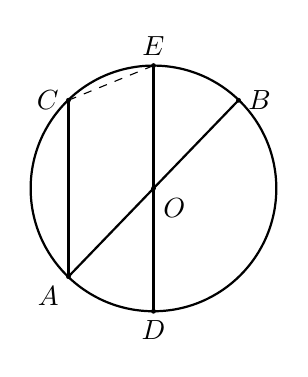
\begin{tikzpicture}[scale=0.8]
  \coordinate (O) at (0,0);
  \coordinate (A) at (-1.35,-1.4);
  \coordinate (B) at (1.35,1.4);
  \coordinate (E) at (0,1.95);
  \coordinate (D) at (0,-1.95);
  \coordinate (C) at (-1.35,1.4);
  \draw[thick] (O) circle (1.95);
  \draw[thick] (A)--(B);
  \draw[thick] (D)--(E);
  \draw[thick] (A)--(C);
  \draw[dashed] (C)--(E);
  \fill (O) circle (1.1pt) node[below right] {$O$};
  \fill (A) circle (1.1pt) node[below left] {$A$};
  \fill (B) circle (1.1pt) node[right] {$B$};
  \fill (C) circle (1.1pt) node[left] {$C$};
  \fill (D) circle (1.1pt) node[below] {$D$};
  \fill (E) circle (1.1pt) node[above] {$E$};
\end{tikzpicture}
\end{center}
\nopagebreak[4]
\Needspace{4\baselineskip}
\textbf{解析}

\gksubpart{（1）}

\Needspace{5\baselineskip}
设储料场沿仓库方向的宽为 $y$，垂直仓库方向的长为 $x$。铁丝网围三边，所以

\nopagebreak[4]
\[
x+2y=50.
\]

\Needspace{5\baselineskip}
面积

\nopagebreak[4]
\[
S=xy=x\frac{50-x}{2}=\frac{25}{2}x-\frac12x^2
=\frac{625}{2}-\frac12(x-25)^2.
\]

故 $x=25$ 米、$y=12.5$ 米时面积最大，最大面积为 $312.5\ \mathrm{m^2}$。

\gksubpart{（2）}

\Needspace{5\baselineskip}
由 $AB\text{、}DE$ 均为直径，圆心 $O$ 分别是 $AB\text{、}DE$ 的中点。因 $AC\parallel DE$，过圆心的直径方向与弦 $AC$ 垂直；结合圆的中心对称，弦 $AC$ 的中点与弦 $DE$ 的对应位置相对称。等价地，平行弦在圆周上截得的对应弧相等，故对应弦

\nopagebreak[4]
\[
CE=EB.
\]

\gkanswer{答案（1）：长 $25$ 米、宽 $12.5$ 米；最大面积为 $312.5\ \mathrm{m^2}$。}

\gkanswer{答案（2）：见解析版}

\end{answer}
\begin{answer}
\gksolhead{3}{}

\textbf{题目}：

如果已知 $bx^2-4bx+2(a+c)=0$（$b\ne0$）有两个相等的实数根，求证：$a\text{、}b\text{、}c$ 成等差数列。

\Needspace{4\baselineskip}
\textbf{解析}

\Needspace{5\baselineskip}
二次方程有两个相等的实根，当且仅当判别式为零：

\nopagebreak[4]
\[
\Delta=(-4b)^2-4b\cdot2(a+c)=0.
\]

\Needspace{5\baselineskip}
因 $b\ne0$，约去 $8b$ 得

\nopagebreak[4]
\[
2b=a+c.
\]

这正是 $a\text{、}b\text{、}c$ 成等差数列的条件。

\gkanswer{答案：见解析版}

\end{answer}
\begin{answer}
\gksolhead{4}{}

\textbf{题目}：

（1） 如图，为求河对岸某建筑物的高 $AB$，在地面上引一条基线 $CD=a$，测得 $\angle ACB=\alpha$，$\angle BCD=\beta$，$\angle BDC=\gamma$，求 $AB$。
\nopagebreak[4]
\begin{center}% 1977 年天津卷第 4(1) 题：河对岸建筑物高度测量
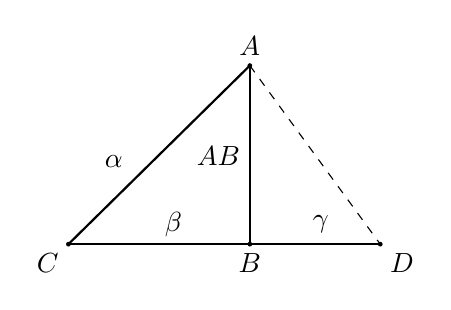
\begin{tikzpicture}[scale=0.72,>=stealth]
  \coordinate (B) at (0.7,0.1);
  \coordinate (A) at (0.7,3.25);
  \coordinate (C) at (-2.5,0.1);
  \coordinate (D) at (3.0,0.1);
  \draw[thick] (A)--(B);
  \draw[thick] (C)--(D);
  \draw[thick] (C)--(A);
  \draw[thick] (C)--(B);
  \draw[thick] (D)--(B);
  \draw[dashed] (A)--(D);
  \fill (A) circle (1.2pt) node[above] {$A$};
  \fill (B) circle (1.2pt) node[below] {$B$};
  \fill (C) circle (1.2pt) node[below left] {$C$};
  \fill (D) circle (1.2pt) node[below right] {$D$};
  \node at (-1.7,1.55) {$\alpha$};
  \node at (-0.65,0.45) {$\beta$};
  \node at (1.95,0.45) {$\gamma$};
  \node[left] at (0.7,1.65) {$AB$};
\end{tikzpicture}
\end{center}
\nopagebreak[4]
（2） 如果 $\alpha=30^\circ$，$\beta=75^\circ$，$\gamma=45^\circ$，$a=33$ 米，求建筑物 $AB$ 的高。（保留一位小数）

\Needspace{4\baselineskip}
\textbf{解析}

\gksubpart{（1）}

\Needspace{5\baselineskip}
在地面三角形 $BCD$ 中，$CD=a$，$\angle BCD=\beta$，$\angle BDC=\gamma$，所以 $\angle CBD=180^\circ-\beta-\gamma$。由正弦定理

\nopagebreak[4]
\[
\frac{BC}{\sin\gamma}=\frac{CD}{\sin(\beta+\gamma)},
\qquad
BC=\frac{a\sin\gamma}{\sin(\beta+\gamma)}.
\]

\Needspace{5\baselineskip}
建筑物 $AB$ 垂直地面，故在直角三角形 $ABC$ 中

\nopagebreak[4]
\[
AB=BC\tan\alpha
=\frac{a\sin\gamma\tan\alpha}{\sin(\beta+\gamma)}.
\]

\gksubpart{（2）}

\Needspace{5\baselineskip}
代入 $\alpha=30^\circ$、$\beta=75^\circ$、$\gamma=45^\circ$、$a=33$：

\nopagebreak[4]
\[
AB=\frac{33\sin45^\circ\tan30^\circ}{\sin120^\circ}
=11\sqrt2\ \mathrm m\approx15.6\ \mathrm m.
\]

\gkanswer{答案（1）：$AB=\dfrac{a\sin\gamma\tan\alpha}{\sin(\beta+\gamma)}$。}

\gkanswer{答案（2）：$AB=11\sqrt2\ \mathrm m\approx15.6\ \mathrm m$。}

\end{answer}
\begin{answer}
\gksolhead{5}{}

\textbf{题目}：

（1） 求直线 $3x-2y+1=0$ 和 $x+3y+4=0$ 的交点坐标。

（2） 求通过上述交点，并同直线 $x+3y+4=0$ 垂直的直线方程。

\begin{gktip}
\Needspace{0.25\textheight}
\textbf{附加题}
\end{gktip}

\Needspace{5\baselineskip}
\textbf{附加题 6．} 求

\nopagebreak[4]
\[
\lim_{x\to0}\frac{\mathrm e^x-\mathrm e^{-x}-2x}{x-\sin nx}
\]

的值。

\Needspace{5\baselineskip}
\textbf{附加题 7．} 计算：

\nopagebreak[4]
\[
\int_0^4\frac{x+2}{\sqrt{2x+1}}\,\mathrm dx.
\]

\Needspace{4\baselineskip}
\textbf{解析}

\gksubpart{（1）}

\Needspace{5\baselineskip}
联立两直线：

\nopagebreak[4]
\[
3x-2y+1=0,\qquad x+3y+4=0.
\]

由第二式 $x=-3y-4$，代入第一式得 $y=-1$，从而 $x=-1$。交点为 $(-1,-1)$。

\gksubpart{（2）}

\Needspace{5\baselineskip}
直线 $x+3y+4=0$ 的斜率为 $-1/3$，垂线斜率为 $3$。过 $(-1,-1)$ 的垂线为

\nopagebreak[4]
\[
y+1=3(x+1),
\]

即 $3x-y+2=0$。

\gksubpart{附加题 6}

\Needspace{4\baselineskip}
\textbf{解析}

\Needspace{5\baselineskip}
在 $x\to0$ 时，

\nopagebreak[4]
\[
\mathrm e^x-\mathrm e^{-x}-2x=\frac{x^3}{3}+o(x^3).
\]

\Needspace{5\baselineskip}
若 $n\ne1$，则

\nopagebreak[4]
\[
x-\sin nx=(1-n)x+O(x^3),
\]

\Needspace{5\baselineskip}
极限为 $0$。若 $n=1$，则

\nopagebreak[4]
\[
x-\sin x=\frac{x^3}{6}+o(x^3),
\]

极限为 $2$。固定源没有给出 $n$ 的取值限制，故只能给出这两个情形。

\gksubpart{附加题 7}

\Needspace{4\baselineskip}
\textbf{解析}

\Needspace{5\baselineskip}
令 $u=\sqrt{2x+1}$，则 $x=(u^2-1)/2$、$\mathrm dx=u\,\mathrm du$。当 $x=0$ 时 $u=1$，当 $x=4$ 时 $u=3$，因此

\nopagebreak[4]
\[
\begin{aligned}
\int_0^4\frac{x+2}{\sqrt{2x+1}}\,\mathrm dx
&=\int_1^3\frac{(u^2-1)/2+2}{u}\,u\,\mathrm du\\
&=\frac12\int_1^3(u^2+3)\,\mathrm du\\
&=\left[\frac{u^3}{6}+\frac{3u}{2}\right]_1^3
=\frac{22}{3}.
\end{aligned}
\]

\gkanswer{答案（1）：$(-1,-1)$。}

\gkanswer{答案（2）：$3x-y+2=0$。}

\end{answer}